% ==========================================
% BAB I PENDAHULUAN
% ==========================================
\chapter{PENDAHULUAN}
\label{chap:pendahuluan}
% --- Latar Belakang ---
\section{Latar Belakang}
% Latar Belakang menjelaskan dasar pemikiran, motivasi, kebutuhan, alasan, atau urgensi pemilihan masalah tugas akhir. Subbab ini berisi penjelasan ringkas tentang kondisi atau situasi yang ada saat ini terkait dengan topik yang dibahas. Tujuan utamanya adalah untuk memberikan informasi secukupnya kepada pembaca agar memahami topik yang akan dibahas. Dalam subbab ini, jelaskan hal-hal berikut ini:
% \begin{enumerate}
% \item	Kondisi atau situasi topik yang dibahas beserta permasalahannya, misalnya tentang pengelolaan informasi di puskesmas daerah pedesaan dan masalah yang dihadapi.
% \item	Berbagai solusi yang telah diterapkan atau solusi yang tersedia dan memungkinkan untuk diterapkan untuk menyelesaikan masalah tersebut.
% \end{enumerate}
Kebutuhan energi listrik pada bangunan gedung terus meningkat seiring bertambahnya aktivitas operasional, penggunaan peralatan listrik, serta tuntutan kenyamanan dan keandalan layanan. Peningkatan ini tidak selalu diimbangi dengan pengelolaan energi yang memadai, sehingga banyak bangunan mengalami konsumsi energi yang tidak efisien. Studi audit energi pada berbagai jenis gedung menunjukkan bahwa ketidakefisienan umumnya disebabkan oleh keterbatasan pemantauan beban listrik, pencatatan data yang tidak berkelanjutan, serta tidak tersedianya dokumentasi kinerja sistem kelistrikan yang terstruktur \cite{hamdani2017audit,winarto2019audit}. Kondisi tersebut berdampak pada tingginya intensitas konsumsi energi (IKE), pemborosan energi listrik, dan berkurangnya kemampuan pengelola gedung dalam mengidentifikasi masalah teknis lebih awal. Hal ini menunjukkan bahwa permasalahan efisiensi energi tidak hanya disebabkan oleh faktor teknis, tetapi juga oleh keterbatasan dalam pengelolaan dan pemanfaatan data energi secara sistematis.

Audit energi merupakan salah satu pendekatan yang banyak digunakan untuk mengatasi permasalahan tersebut. Audit energi dilakukan melalui proses evaluasi sistematis terhadap pola pemakaian energi, pengukuran parameter kelistrikan, serta analisis indikator kinerja energi untuk mengidentifikasi peluang penghematan. Pelaksanaan audit energi umumnya mengacu pada standar dan pedoman yang telah ditetapkan, seperti ISO 50001 yang mengatur kerangka sistem manajemen energi, ISO 50002 yang memberikan panduan teknis audit energi, serta SNI 03-6196-2000 yang menjadi acuan nasional audit energi pada bangunan gedung \cite{iso2018_50001,iso2014_50002,sni2000_036196}. Penelitian terdahulu menunjukkan bahwa audit energi yang dilakukan secara terstruktur mampu memberikan gambaran kuantitatif kondisi konsumsi energi dan menjadi dasar perencanaan tindakan efisiensi \cite{putra2025evaluasi}.

Namun, dalam praktiknya, proses audit energi pada banyak bangunan masih dilakukan secara manual dengan mengandalkan pencatatan lapangan, pengolahan data menggunakan \textit{spreadsheet}, serta perhitungan indikator secara terpisah. Pendekatan ini rentan terhadap kesalahan input, inkonsistensi metode perhitungan, dan kesulitan dalam menelusuri kembali hasil audit terdahulu. Beberapa penelitian menunjukkan bahwa pemanfaatan perangkat lunak sederhana, seperti sistem audit IKE berbasis antarmuka grafis, dapat membantu mengotomasi perhitungan dan mengurangi beban kerja auditor, meskipun fungsinya masih terbatas pada aspek tertentu \cite{fitri2022sistem}. Pengembangan sistem informasi untuk pengelolaan fasilitas gedung juga terbukti meningkatkan keteraturan data dan mendukung proses pengambilan keputusan teknis, meskipun belum secara spesifik dirancang untuk audit energi \cite{hermawan2022perencanaan}. Dengan demikian, masih terdapat kesenjangan dalam pengembangan sistem yang mampu mengintegrasikan proses pengumpulan data, perhitungan indikator energi, serta pemenuhan standar audit dalam satu platform yang terpadu.

Kajian mengenai sistem pendukung audit menegaskan bahwa penggunaan perangkat lunak dapat meningkatkan konsistensi proses, kualitas dokumentasi, dan keandalan hasil evaluasi, selama sistem dirancang untuk mendukung alur kerja audit dan tetap memberikan ruang bagi penilaian profesional auditor \cite{dowling2007audit}. Oleh karena itu, diperlukan suatu perangkat lunak penilaian audit energi yang tidak hanya mampu mengotomasi perhitungan indikator kinerja energi, tetapi juga mendukung kepatuhan terhadap standar audit, menyediakan dokumentasi yang terstruktur, serta memudahkan analisis dan pelaporan hasil audit secara terintegrasi.

Berdasarkan kondisi tersebut, pengembangan perangkat lunak penilaian audit energi pada bangunan gedung menjadi kebutuhan yang relevan dan mendesak. Selain itu, sistem yang dikembangkan diharapkan mampu mengatasi keterbatasan proses audit energi konvensional yang masih bersifat manual dan tidak terintegrasi.

% --- Rumusan Masalah ---
\section{Rumusan Masalah}
% Rumusan Masalah berisi masalah utama yang dibahas dalam tugas akhir. Rumusan masalah yang baik memiliki struktur sebagai berikut:
Berdasarkan latar belakang yang sudah dijelaskan diperoleh beberapa rumusan masalah sebagai berikut.

\begin{enumerate}
    \item Bagaimana kondisi sistem kelistrikan gedung saat ini dalam hal pemantauan, pencatatan, dan evaluasi konsumsi energi, mengingat masih terbatasnya instrumen pengukuran permanen dan keterbatasan akurasi audit manual?
    \item Bagaimana merancang suatu sistem atau perangkat lunak penilaian yang mampu mendukung proses audit energi agar lebih cepat, terstandar, dan reliabel, sejalan dengan praktik dan rekomendasi sistem audit berbasis perangkat lunak yang telah diteliti sebelumnya?
    \item Bagaimana efektivitas perangkat lunak dalam mendukung kepatuhan proses audit energi terhadap persyaratan standar ISO 50001, ISO 50002, dan SNI 03-6196-2000 pada studi kasus satu gedung?
\end{enumerate}

% --- Tujuan ---
\section{Tujuan}
Berdasarkan permasalahan dan rumusan masalah, maka tujuan dari dilakukannya penelitian ini adalah sebagai berikut.

\begin{enumerate}
    \item Mengkaji dan mendeskripsikan kondisi sistem kelistrikan gedung terkait proses pemantauan, pencatatan, serta evaluasi konsumsi energi yang masih dilakukan secara manual.
    \item Merancang dan mengembangkan sebuah perangkat lunak penilaian yang mampu mendukung proses audit energi secara lebih cepat, terstandar, dan reliabel melalui fasilitas perhitungan indikator, visualisasi data, dan penyusunan laporan otomatis.
    \item Mengevaluasi kemampuan perangkat lunak untuk mendukung pemenuhan persyaratan audit energi sesuai ISO 50001, ISO 50002, dan SNI 03-6196-2000 dengan mengukur tingkat kepatuhan checklist standar, kesesuaian format laporan, dan kelengkapan dokumentasi bukti audit pada studi kasus satu gedung.
\end{enumerate}

% --- Batasan Masalah ---
\section{Batasan Masalah}
Untuk menjaga fokus dari tugas akhir ini, ditetapkan beberapa batasan masalah yang akan diterapkan selama pembuatan tugas akhir ini yaitu sebagai berikut.

\begin{enumerate}
    \item Sumber data yang digunakan dalam perangkat lunak ini berasal dari hasil input manual.
    \item Evaluasi kepatuhan terhadap standar dibatasi pada aspek audit energi yang berkaitan dengan metodologi audit, indikator kinerja energi, format pelaporan, dan dokumentasi audit sesuai ISO 50001, ISO 50002, dan SNI 03-6196-2000.
\end{enumerate}

% --- Metodologi Pengerjaan TA ---
\section{Metodologi}
Metodologi yang digunakan dalam tugas akhir ini adalah metode pengembangan perangkat lunak Waterfall. Metode ini dipilih karena kebutuhan sistem audit energi relatif jelas dan stabil serta mengacu pada standar audit energi yang telah ditetapkan. Pengembangan perangkat lunak dilakukan secara bertahap dan terstruktur mulai dari analisis kebutuhan hingga pemeliharaan sistem. Pendekatan ini memungkinkan dokumentasi yang jelas pada setiap tahap serta memudahkan proses evaluasi terhadap kesesuaian sistem dengan kebutuhan pengguna dan persyaratan standar \cite{sommerville2016software}. Alur tahapan metodologi Waterfall yang digunakan dalam penelitian ini ditunjukkan pada diagram Gambar \ref{gambar:waterfall}.

\begin{figure}[H] % pilihan opsi yang disarankan: H = here (requires float package)
    \centering
    \captionsetup{justification=centering}
        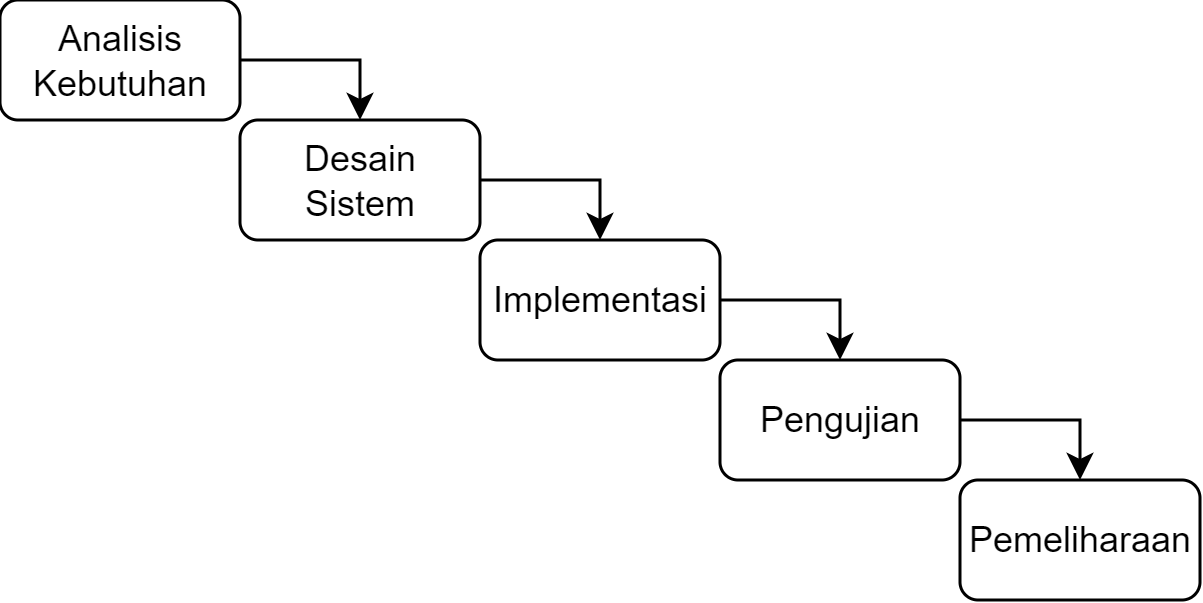
\includegraphics[width=0.7\textwidth]{image/waterfall}
    \caption{Tahapan \textit{Waterfall} Sesuai Sommerville \cite{sommerville2016software}}
    \label{gambar:waterfall}
\end{figure}

Tahapan pengembangan perangkat lunak dalam penelitian ini dijabarkan sebagai berikut.

\begin{enumerate}
    \item Analisis Kebutuhan
    
    Tahap ini bertujuan untuk mengidentifikasi kebutuhan perangkat lunak audit energi berdasarkan kondisi proses audit yang berjalan saat ini. Kegiatan pada tahap ini meliputi analisis proses audit manual, studi literatur terkait audit energi dan standar yang digunakan, wawancara dan/atau observasi dengan auditor energi serta pengelola gedung, serta perumusan kebutuhan fungsional dan nonfungsional sistem.

    \vspace{.1cm}
    \item Desain Sistem
    
    Tahap ini bertujuan untuk merancang solusi sistem berdasarkan kebutuhan yang telah ditetapkan. Perancangan mencakup desain fungsional, desain data, serta desain perilaku sistem yang menggambarkan alur proses dan respons sistem terhadap kejadian. Hasil tahap ini menjadi acuan utama dalam proses implementasi perangkat lunak.
    
    \vspace{.1cm}
    \item Implementasi
    
    Tahap ini bertujuan untuk membangun perangkat lunak sesuai dengan desain sistem yang telah dirancang. Implementasi meliputi pengembangan modul input data audit, pemrosesan dan perhitungan indikator kinerja energi, mekanisme sinkronisasi data, serta penyajian hasil audit dalam bentuk \textit{dashboard} dan laporan otomatis.
    
    \vspace{.1cm}
    \item Pengujian
    
    Tahap ini bertujuan untuk memastikan kesesuaian fungsi dan kinerja sistem dengan kebutuhan yang telah ditetapkan. Pengujian meliputi pengujian fungsional setiap modul, verifikasi akurasi perhitungan indikator kinerja energi, serta pengujian alur proses audit menggunakan data studi kasus. Selain itu, dilakukan pengujian nonfungsional untuk menilai aspek kegunaan, keandalan, dan kinerja sistem.

    \vspace{.1cm}
    \item Pemeliharaan
    
    Tahap ini bertujuan untuk menjaga stabilitas dan keberlanjutan penggunaan perangkat lunak. Kegiatan pemeliharaan meliputi perbaikan kesalahan yang ditemukan selama pengujian dan penggunaan awal sistem, serta penyesuaian minor untuk meningkatkan stabilitas dan kegunaan perangkat lunak berdasarkan hasil evaluasi dan umpan balik pengguna.
\end{enumerate}
% Metodologi yang digunakan dalam penelitian ini adalah pengembangan desain interaksi berdasarkan pendekatan \textit{User Centered Design} sesuai ISO 9241-210:2019 \cite{iso2019_9241_210}. Pendekatan ini menempatkan pengguna sebagai pusat proses desain dan dilakukan secara iteratif melalui siklus pemahaman konteks, perumusan kebutuhan, perancangan, dan evaluasi. Gambar \ref{gambar:ucd} menggambarkan tahapan utama pendekatan ini.

% \begin{figure}[H] % pilihan opsi yang disarankan: H = here (requires float package)
%     \centering
%     \captionsetup{justification=centering}
%         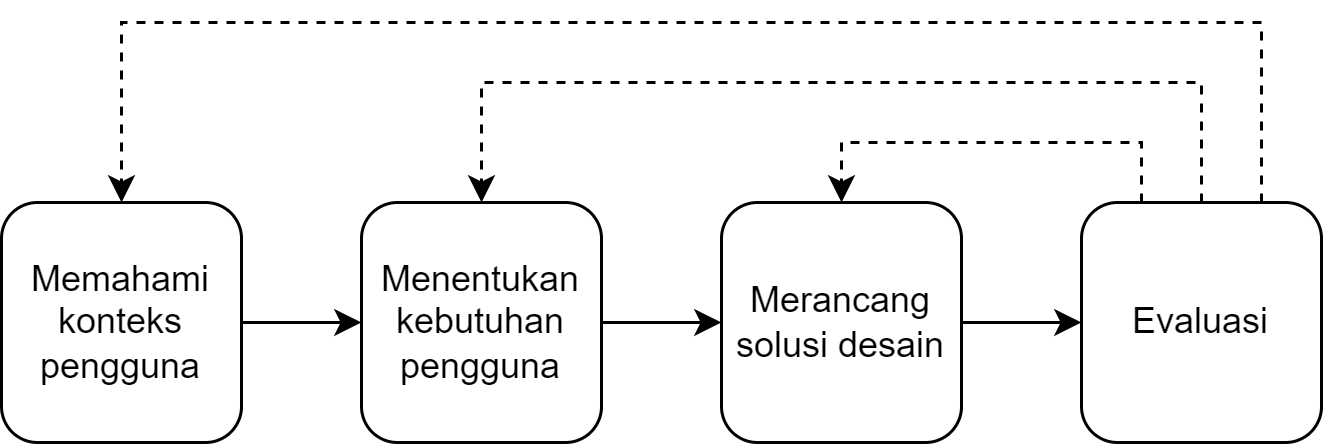
\includegraphics[width=0.7\textwidth]{image/ucd}
%     \caption{Tahapan \textit{User Centered Design} Sesuai ISO 9241-210:2019}
%     \label{gambar:ucd}
% \end{figure}

% \begin{enumerate}
%     \item Memahami konteks penggunaan.
  
%     Mengidentifikasi pengguna utama, tugas, tujuan penggunaan, dan lingkungan operasional perangkat lunak audit energi. Kegiatan meliputi studi literatur, pengumpulan contoh data, serta wawancara atau observasi dengan auditor energi dan pengelola gedung.

%     \item Menentukan kebutuhan pengguna
    
%     Menentukan  kebutuhan fungsional dan nonfungsional. Hasilnya berupa daftar user requirements dan skenario penggunaan yang akan menjadi dasar desain.

%     \item Merancang solusi desain (iterasi pertama)
    
%     Membuat diagram, \textit{wireframe}, dan prototipe \textit{low fidelity} yang menampilkan alur utama sistem, yaitu, input data, perhitungan indikator, penilaian, visualisasi, dan laporan.

%     \item Evaluasi (iterasi pertama)
    
%     Melakukan uji kegunaan dengan tugas terstruktur pada prototipe serta mengumpulkan metrik kualitatif dan kuantitatif serta umpan balik pengguna untuk perbaikan.

%     \item Merancang solusi desain (iterasi kedua).
    
%     Membuat prototipe menjadi versi lebih matang (\textit{high fidelity}) berdasarkan hasil uji pertama, perbaiki alur dan elemen antarmuka.

%     \item Evaluasi (iterasi kedua).
    
%     Menguji ulang dengan pengguna yang serupa untuk menilai apakah perbaikan memenuhi kebutuhan pengguna.

%     \item Merancang solusi desain (iterasi ketiga)
    
%     Melakukan penyempurnaan akhir pada desain dan lanjutkan ke implementasi modul fungsional perangkat lunak.
    
%     \item Evaluasi (iterasi ketiga)
    
%     Memvalidasi fungsi dan akurasi perhitungan menggunakan studi kasus serta melakukan pengujian kegunaan akhir dan mendokumentasikan temuan serta rekomendasi pengembangan lanjutan.
% \end{enumerate}